\documentclass[a4paper, 12pt]{article}
\usepackage[T2A]{fontenc}
\usepackage[utf8]{inputenc}
\usepackage[english,russian]{babel}
\usepackage{amsmath, amsfonts, amssymb, amsthm, mathtools, misccorr, indentfirst, multirow}
\usepackage{wrapfig}
\usepackage{graphicx}
\usepackage{subfig}
\usepackage{adjustbox}
\usepackage{pgfplots}

\usepackage{geometry}
\geometry{top=20mm}
\geometry{bottom=20mm}
\geometry{left=20mm}
\geometry{right=20mm}
\newcommand{\angstrom}{\textup{\AA}}
\begin{document}
	\begin{titlepage}
		\begin{center}
		МИНИСТЕРСТВО ОБРАЗОВАНИЯ И НАУКИ РОССИЙСКОЙ ФЕДЕРАЦИИ\\
		\footnotesize{Московский физико-технический институт}\\
		\footnotesize{(государственный университет)}\\
		\footnotesize{Кафедра вакуумной электроники}\\
		\vfill
		{\LARGE
		\textbf{Растровый электронный микроскоп}\\
		}
		\vspace{1cm}
		Лабораторная работа по курсу\\
		вакуумная электроника
		\vfill
		\begin{flushright}
			Выполнил: студент 654гр.\\
			Нехаев А.С.
		\end{flushright}
		\vfill
		г. Долгопрудный\\
		2018 год
		\end{center}
	\end{titlepage}
	\newpage
	\pagenumbering{arabic}
	\tableofcontents
	\newpage
	\section{Введение}
	Растровый электронный микроскоп (РЭМ) является одним из основных средств проведения измерений в нанометровой области. Данная лабораторная работа направлена на ознакомление физическими принципами функционирования РЭМ и основными методиками измерения.
	\section{Цели и задачи исследования}
	\begin{enumerate}
		\item Получить изображение образца в различных режимах работы микроскопа:
		\begin{enumerate}
			\item в режиме сбора истинно вторичных электронов (SE);
			\item в режиме сбора упруго отраженных электронов (BSE);
		\end{enumerate}
		\item Получить изображение образца в высоком и низком вакууме;
		\item Изучить физические принципы формирования изображений в растровом электронном микроскопе;
		\item Применить рентгеновский микроанализ для определения элементного состава образца;
	\end{enumerate}
	\newpage
	\section{Основная часть}
	Микроскоп, изучаемый в ходе данной работы, позволяет вести наблюдения образца в трех основных режимах: во вторичных электронах, в отраженных электронах, в рентгеновских лучах (микроанализатор). Для первых двух режимов оптимальный ток с точки зрения точности результатов составляет 1-1000 пА, при рентгеновском микроанализе оптимальным считается ток зонда порядка 100 нА. Поэтому ток зонда микроскопа варьируется в широких пределах.\par
	Образец крепится в специальном держателе, позволяющем максимально удобно оперировать с образцами в процессе работы. Образец окружен детектирующей аппаратурой - детектором отражённых электронов, детектором вторичных электронов.\par
	Помимо колонны, в виде отдельных блоков смонтирована остальная аппаратура - это вакуумная система, счетный блок рентгеновского спектрометра и компьютер, позволяющий считывать результаты наблюдений и управлять системой в целом.\par
	\begin{figure}[h]
		\centering
		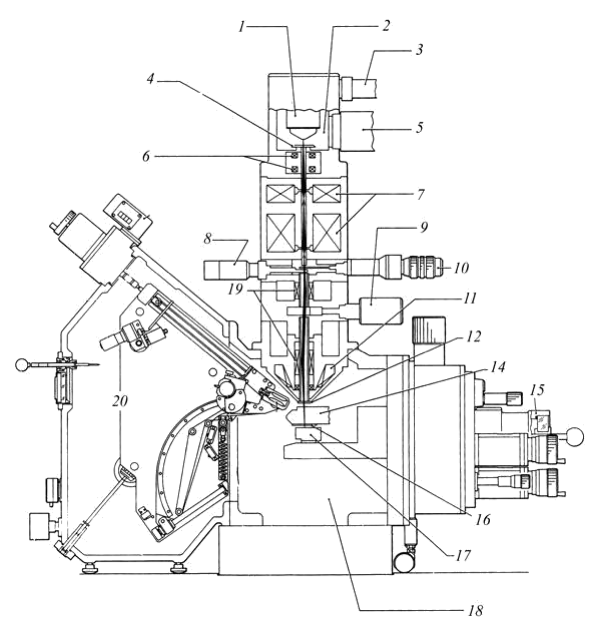
\includegraphics{Microscope_schematic}
		\caption{Общая схема электронно-растрового микроскопа\\
		1 –- электронная пушка; 2 -- камера электронной пушки; 3 -- высоковольтный кабель; 4 -- анод; 5 -- вакуумная магистраль; 6 -- юстировочные катушки; 7 -- конденсорные линзы; 8 -- измеритель тока пучка; 9 -- вакуумный клапан;  9 -- вакуумный клапан; 10 -- устройство выбора диафрагм; 11 -- объектная линза; 12,16 -- детектор упруго отраженных электронов; 14 -- оптический микроскоп; 15 -- шлюз для замены образцов; 17 -- держатель образцов; 18 -- основная вакуумная камера; 19 -- сканирующие катушки; 20 -- рентгеновский спектрометр.
		}
		\label{microscope_scheme}
	\end{figure}
	\subsection{Примеры полученных изображений}
	Сначала получим изображения микросхемы операционного усилителя в режиме сбора истинно вторичных электронов (рис. \ref{fig:iv_001}). Точно также сделаем снимки в топографическом контрасте (рис. \ref{fig:topo_001}) и в режиме z-контраста (рис. \ref{fig:z_001}).\par
	\begin{figure}[!htb]
		\minipage{0.32\textwidth}
			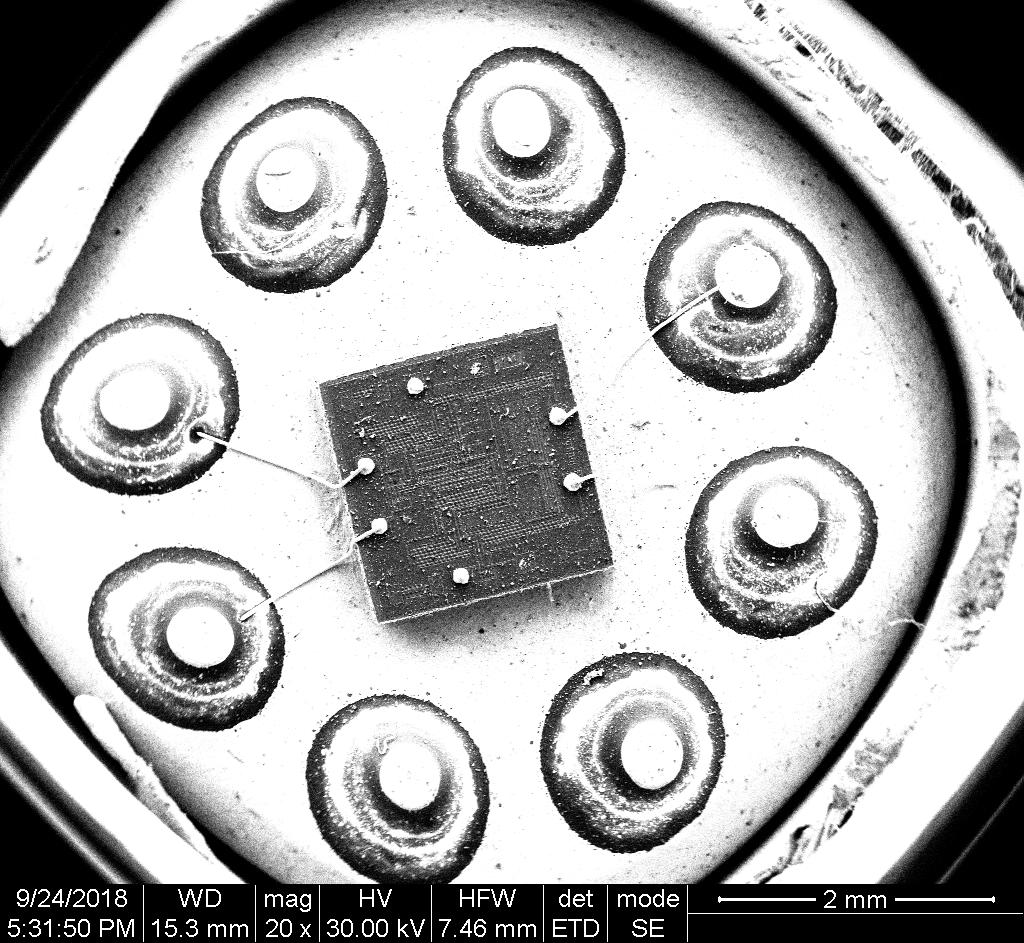
\includegraphics[width=\linewidth]{iv_001.jpg}
			\caption{Изображение микросхемы в режиме сбора истинно вторичных электронов}
			\label{fig:iv_001}
		\endminipage\hfill
		\minipage{0.32\textwidth}
			\includegraphics[width=\linewidth]{a_001.tif}
			\caption{Изображение микросхемы в режиме сбора истинно вторичных электронов}
		\endminipage\hfill
		\minipage{0.32\textwidth}
			\includegraphics[width=\linewidth]{b_001.tif}
			\caption{Изображение микросхемы в режиме сбора истинно вторичных электронов}
		\endminipage
	\end{figure}
	\begin{figure}[!htb]
		\minipage{0.32\textwidth}
			\includegraphics[width=\linewidth]{topo_001.tif}
			\caption{Изображение микросхемы в режиме топографического контраста}
			\label{fig:topo_001}
		\endminipage\hfill
		\minipage{0.32\textwidth}
			\includegraphics[width=\linewidth]{z_001.tif}
			\caption{Изображение микросхемы в режиме z-контраста}
			\label{fig:z_001}
		\endminipage
	\end{figure}
	На рисунке \ref{fig:iv_005} представлен медь-хром образец в режиме сканирования истинно-вторичных электронов. На рисунке \ref{fig:topo_004} представлен тот же образец в режиме топографического контраста. Наиболее информативным является рис. \ref{fig:z_004}, на нем видные распределения различных элементов в образце.\par
	\begin{figure}[!htb]
		\minipage{0.32\textwidth}
		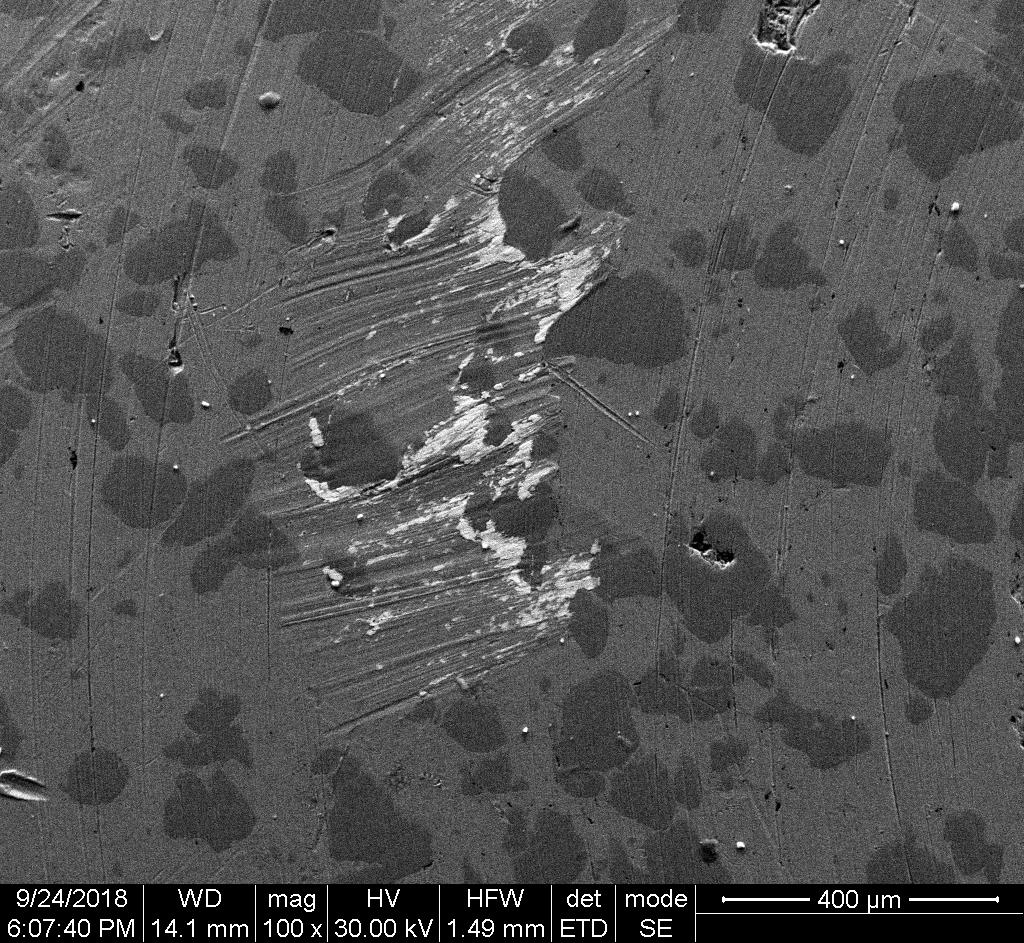
\includegraphics[width=\linewidth]{iv_005.jpg}
		\caption{Изображение медь-хром образца в режиме сбора истинно-вторичных электронов}
		\label{fig:iv_005}
		\endminipage\hfill
		\minipage{0.32\textwidth}
		\includegraphics[width=\linewidth]{topo_004.tif}
		\caption{Изображение медь-хром образца в топографическом режиме}
		\label{fig:topo_004}
		\endminipage\hfill
		\minipage{0.32\textwidth}
		\includegraphics[width=\linewidth]{z_004.tif}
		\caption{Изображение медь-хром образца в режиме z-контраста}
		\label{fig:z_004}
		\endminipage
	\end{figure}
	Далее получим изображение диэлектрика. В нашем случае это кусочек пенопласта. В силу своих свойств он будет работать как зеркало и мы сможем увидеть содержимое камеры. Сперва зарядим поверхность диэлектрика мощным пучком электронов. Поскольку изображение снимается в вакууме, заряд с него уйти не может и поверхность начнет отражать падающий на неё пучок с меньшей энергией. На рисунке \ref{fig:iv_006} представлено изображение камеры, полученное при съемке диэлектрика в режиме истинно-вторичных электронов.
	\begin{figure}[!htb]
		\minipage{0.48\textwidth}
		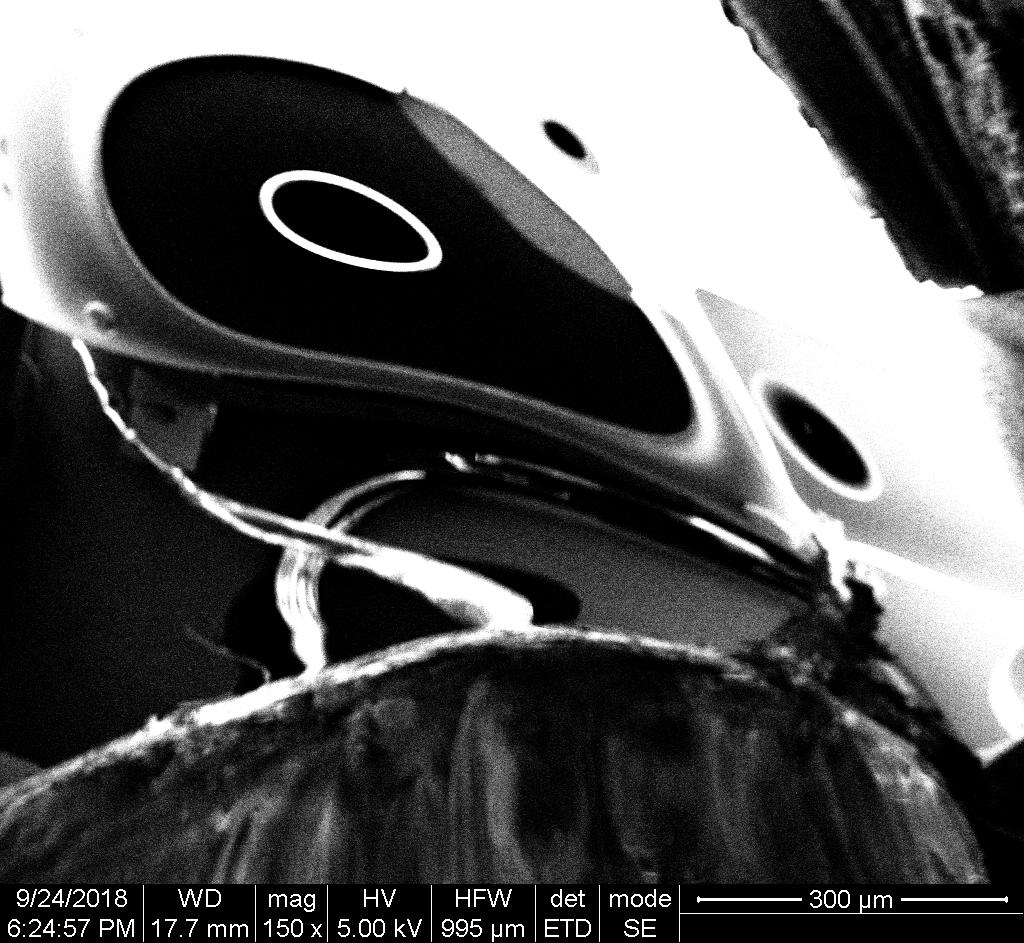
\includegraphics[width=\linewidth]{iv_006.jpg}
		\caption{Изображение диэлектрика в режиме сбора истинно-вторичных электронов}
		\label{fig:iv_006}
		\endminipage\hfill
		\minipage{0.48\textwidth}
		\includegraphics[width=\linewidth]{topo_005.tif}
		\caption{Изображение диэлектрика в топографическом режиме}
		\label{fig:topo_005}
		\endminipage
	\end{figure}
	На рисунке \ref{fig:topo_005} изображен снимок диэлектрика в топографическом режиме. На нем хорошо виден парный детектор и две его половины. Обратим внимание, что разные его половины имеют разные цвета из-за того, что сканер находится в режиме съемки отраженных электронов.\par
	\begin{figure}[!htb]
		\minipage{0.48\textwidth}
		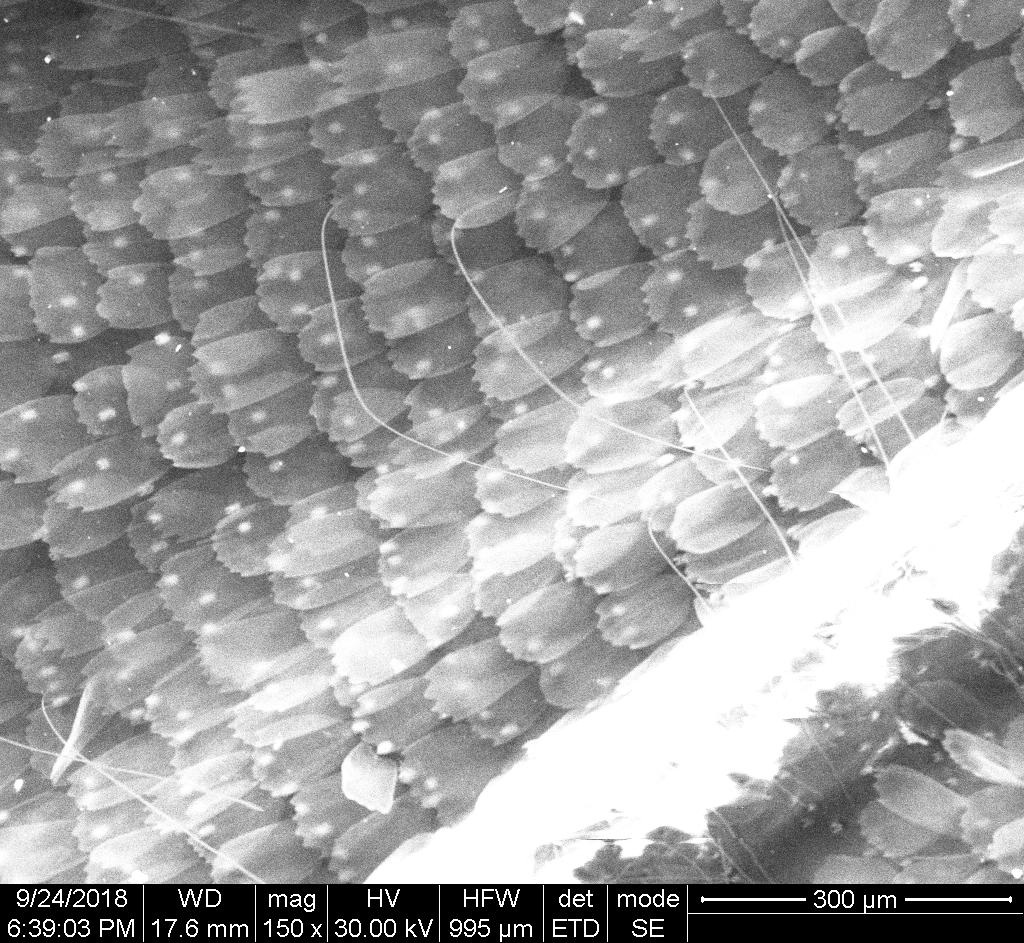
\includegraphics[width=\linewidth]{iv_011.jpg}
		\caption{Изображение крыла бабочки в режиме сбора истинно-вторичных электронов}
		\endminipage\hfill
		\minipage{0.48\textwidth}
		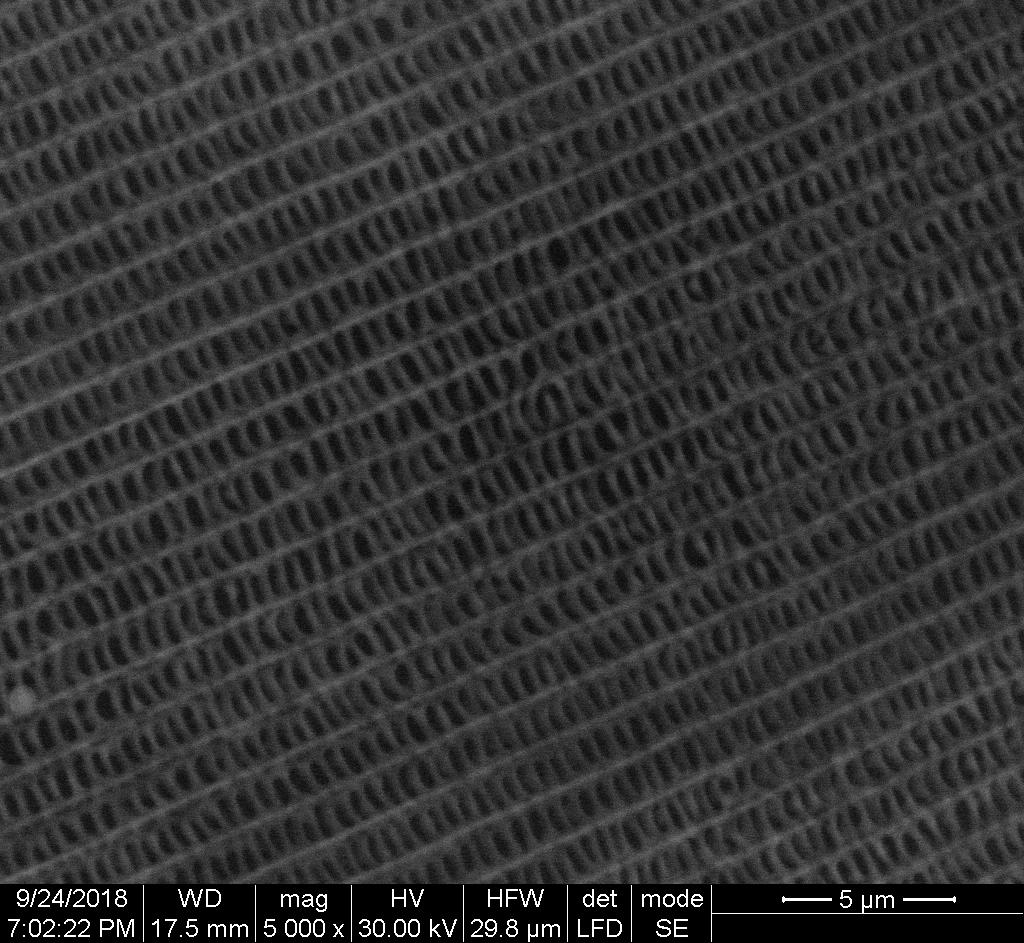
\includegraphics[width=\linewidth]{iv_013.jpg}
		\caption{Изображение крыла бабочки в режиме сбора истинно-вторичных электронов}
		\endminipage
	\end{figure}
	Как видно из снимков крыла бабочки (органический образец), для того, чтобы получить снимок диэлектрика, достаточно понизить вакуум для того чтобы чтобы было достаточное число газа для удаления избыточного заряда.
	\newpage
	\section{Вывод}
	Удалось в процессе работы познакомиться с различными режимами работы РЭМ и некоторыми его особенностями. В ходе работы были получены изображения как проводящих, так и органических образцов, а так же исследован сам зонд и поверхность камеры. Так же мы предприняли попытки объяснить некоторые искажения в работе прибора на основе физических принципов работы микроскопа.
\end{document}